\documentclass{beamer}
\usetheme[pageofpages=of,% String used between the current page and the
                         % total page count.
          bullet=circle,% Use circles instead of squares for bullets.
          titleline=true,% Show a line below the frame title.
          alternativetitlepage=true,% Use the fancy title page.
       %   titlepagelogo=logo-polito,% Logo for the first page.
       %   watermark=watermark-polito,% Watermark used in every page.
       %   watermarkheight=100px,% Height of the watermark.
       %   watermarkheightmult=4,% The watermark image is 4 times bigger
                                % than watermarkheight.
          ]{Torino}

\setbeamertemplate{footline}{
  \begin{beamercolorbox}[wd=\paperwidth,ht=1ex,dp=1ex]{footline}
    \vspace{5pt} \hspace{1em} \insertframenumber/\inserttotalframenumber
  \end{beamercolorbox}
}

\author{Brendon J. Brewer}
\title{STATS 331 -- Introduction to Bayesian Statistics}
\institute{The University of Auckland}
\date{}


\linespread{1.3}
\usepackage{minted}
\usepackage[utf8]{inputenc}
\usepackage{dsfont}


\begin{document}

\frame{\titlepage}

\begin{frame}
\centering
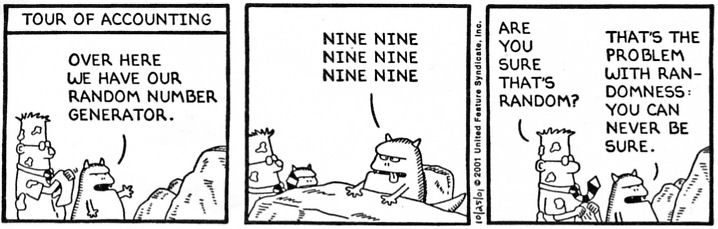
\includegraphics[width=0.8\textwidth]{images/dilbert.jpg}

\end{frame}



\begin{frame}
\centering
\large
Bayesian Linear Regression

\end{frame}


\begin{frame}
\frametitle{Models}
\begin{itemize}
\item We have seen most of the fundamental principles that we will need
throughtout the course.\pause
\item From now on, most of what we will study are particular `models'
for common data analysis situations.\pause
\item We will start with simple linear regression.
\end{itemize}

\end{frame}



\begin{frame}
\frametitle{Road Sign Data}
\centering
\includegraphics[width=0.8\textwidth]{images/road_data.pdf}
\end{frame}



\end{document}

